\section{Charged Kaon Decays at the Super Proton Synchrotron}
\label{sec:na48_na62_experiment}
NA48/2~\cite{Batley:1999fv} and NA62~\cite{Martellotti:2015kna} (also known as NA48/3) are two experiments studying rare kaon decays at the CERN SPS\@.
Each experiment has its own objective, but both study kaon decays and have a dedicated $K^+$ beam, which we can take advantage of for the purpose of setting limits.
Note that the beam is actually a simultaneous $K^+$ and $K^-$ beam, but there are some advantages that make the $K^+$ beam more desirable.
The charged kaon beam is produced similarly to the muon beam that was described in the previous section.
Protons are collided with targets that produce a secondary beam, which are steered towards a target after being selected to ensure that the beam content is purely kaons.
Beryllium is used as for the target, and the beam is a $400~\textrm{GeV}$ proton beam.

\subsection{NA48/2}
NA48/2 finished taking data in 2004, yet limits on new physics can still be derived using the data collected and stored on tape.
NA48/2 is based on the upgraded NA48 experiment, and was primarily designed to look for charge-parity (CP) violation in the decays of charged kaons:

\begin{align}
K^\pm & \rightarrow \pi^+ + \pi^- + \pi^\pm \\
    K^\pm & \rightarrow \pi^0 + \pi^0 + \pi^\pm \textrm{.}
\end{align}

The experiment collected $1.0 \times 10^{11}$ $K^+$ decays inside its fiducial volume during the running time from $2003-2004$.
The data stored on tape is still being used to put some of the most competitive limits on the dark photon parameter space, and has recently ruled it out as a candidate for the resolution of the $(g-2)_\mu$ discrepancy~\cite{Goudzovski:2014rwa}.
For the majority of this analysis, we will be treating NA48/2 as the NA62 experiment with a scaled down number of kaons decaying in the fiducial volume.

\subsection{NA62}
NA62 is looking to measure the Cabbibo-Kobayashi-Maskawa (CKM) matrix element $|V_{td}|$ at the level of $10\%$ by measuring the very rare charged kaon decay:
\begin{equation}
K^+ \rightarrow \pi^+ + \nu + \bar{\nu}
\end{equation}
The SM branching ratio has been determined to be $\textrm{BR}(K^+ \rightarrow \pi^+ + \nu + \bar{\nu}) = (7.81 \pm 0.75 \pm 0.29) \times 10^{-11}$, with the first uncertainty being due to the input parameters, and the second uncertainty coming from theory~\cite{Straub:2010ih}.
Precise measurements of this branching ratio should allow one to put strong limits on any new physics involving the charged kaons.
In October 2014, NA62 successfully launched and began taking data.
It is expected to collect $4.5 \times 10^{12}$ $K^+$ decays within the fiducial volume for each year of running at the SPS\@.

Different than the previous experiments, NA62 is analyzing kaon decays while they are in flight $75~\textrm{GeV}$ $K^+$ beam.
This beam momentum is well defined, having an error of $1\%$.
The liquid krypton (LKr) electro-magnetic calorimeter is reused from the NA48 experiments and is placed past the fiducial volume, giving a coverage of $8.5~\textrm{mrad}$ from the beam.
New to this experiment are the Muon Veto (MUV) and the Large-Angle Photon Vetoes (LAV).
The LAV provides coverage from the LKr limit of $8.5~\textrm{mrad}$ up to $50~\textrm{mrad}$, and has an inefficiency of $10^{-3} - 10^{-4}$ of detecting photons with energies down to $150~\textrm{MeV}$.
The MUV is used to reject muons, which is also handled by the Ring Imaging CHerenkov (RICH) detector.
There are many other important components to the experiment, but the most important things that we must consider are the beam momentum, the LKr calorimeter, and the photon veto efficiency.
To estimate relevant backgrounds, we need to know the probability of not detecting a photon, the efficiency at which the events will hit the LKr calorimeter, and the energy resolution, which is quoted at $\frac{\sigma_E}{E} = \sqrt{\left(\frac{3.2\%}{E^{1/2}}\right)^2 + \left(\frac{9\%}{E}\right)^2 + (0.42\%)^2}$ with $E$ measured in $\textrm{GeV}$.

A schematic view of the experiment is laid out in Fig.~\ref{fig:na62_experiment}.

\begin{figure}[h]
    \centering
    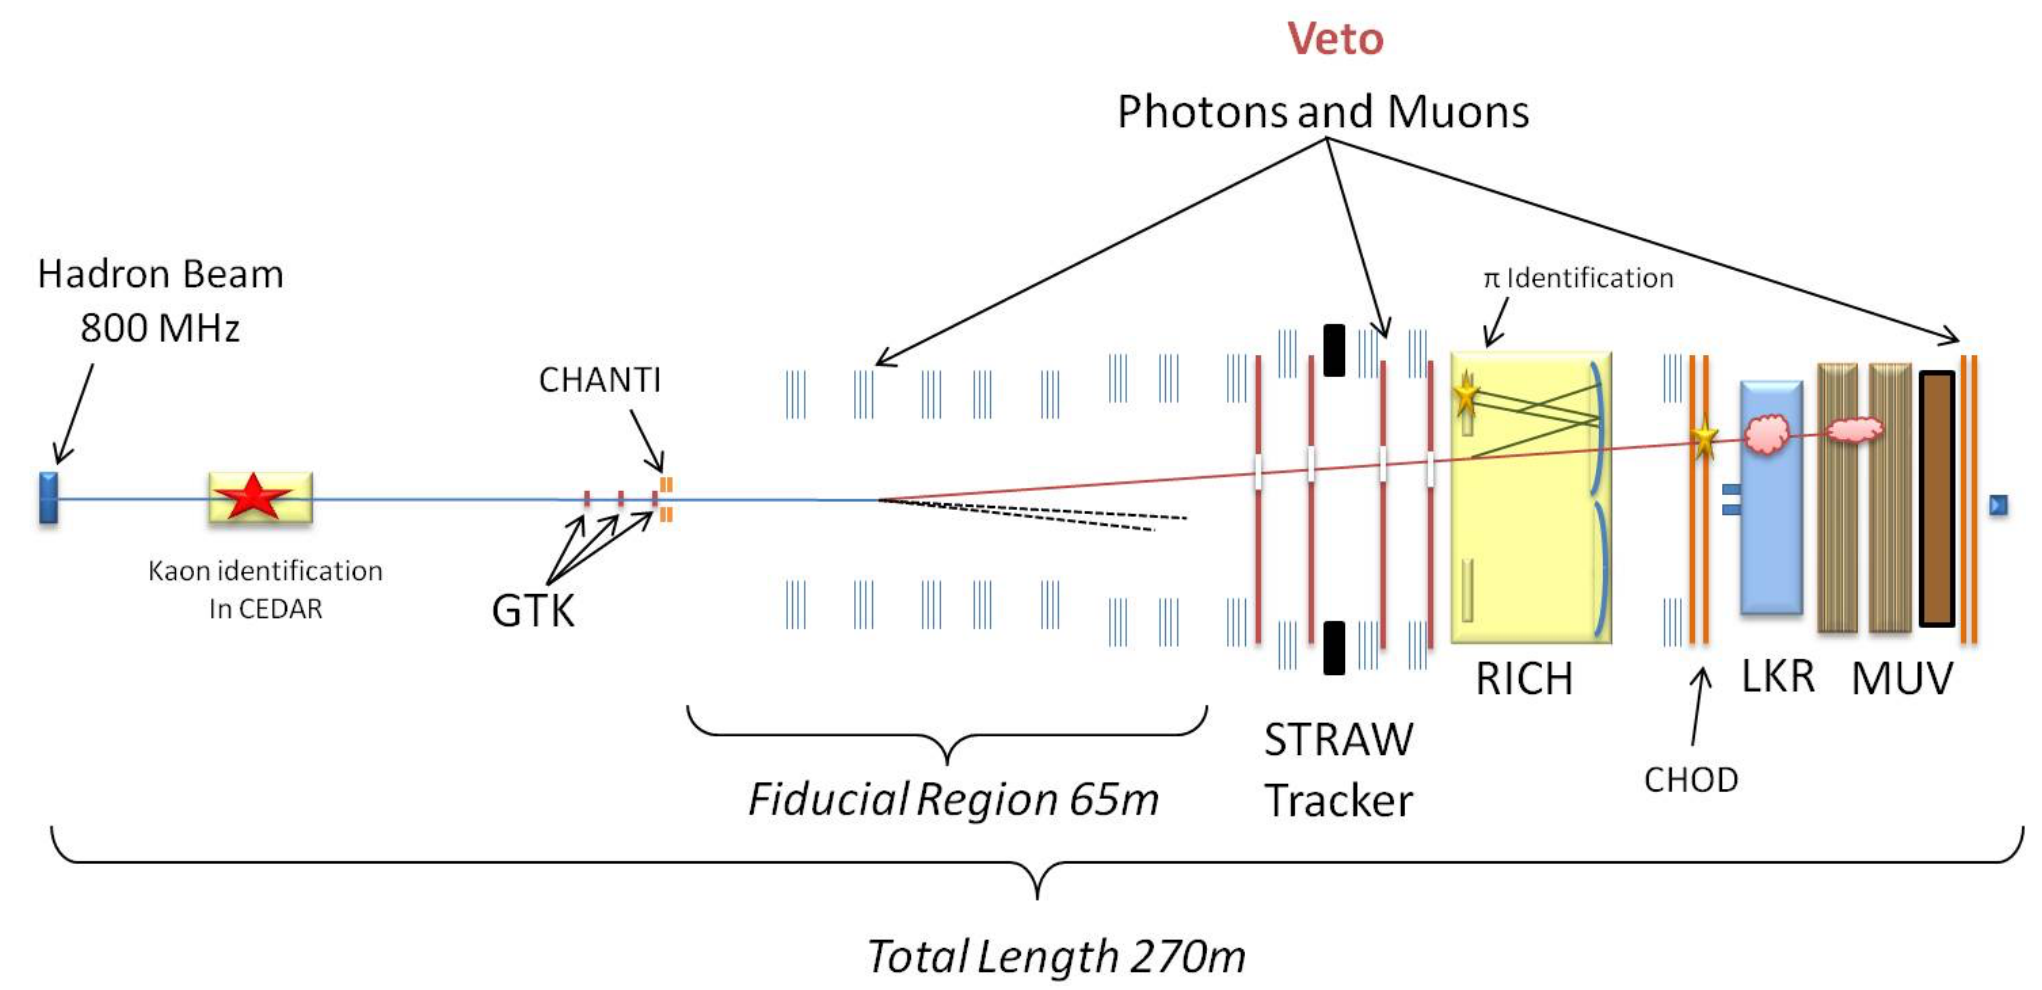
\includegraphics[width=\textwidth]{Figures/experiments/na62_schematic}
    \caption{Schematic of the NA62 experiment from~\cite{Martellotti:2015kna}. The beam collides with a beryllium target and kaons are identified. $K^+$ decays that are visible will decay within the fiducial volume and be captured by the LKr calorimeter. Beyond that, photons can be captured and vetoed outside of the calorimeter.}
    \label{fig:na62_experiment}
\end{figure}

One advantage to using a $K^+$ beam over a $K^-$ beam is that the production rate is $K^+ / K^- \approx 2.1$ higher for each $400\textrm{GeV}$ proton striking the target, while the relative number of pions created, compared to that of a $K^-$ beam, is only $(K^+ / \pi^+) / (K^- / \pi^-) \approx 1.2$.
